\documentclass{report}

% Misc packages
\usepackage{amsmath}
\usepackage{graphicx}
\usepackage{multirow}

% Better font
\usepackage[protrusion=true,expansion=true]{microtype}
\usepackage[T1]{fontenc}
\usepackage{pxfonts}

% Clickable links
\usepackage{hyperref}
\hypersetup{
    colorlinks,
    citecolor=black,
    filecolor=black,
    linkcolor=black,
    urlcolor=black
}

% bibtex stuff
\usepackage{natbib}
\bibliographystyle{abbrvnat}

% Custom Commands
\newcommand{\degree}{\ensuremath{^\circ}}
\newcommand{\todo}{\textbf{TODO} }

\title{Literature Review of Point Cloud Compression}
\author{Keegan Smith\\ksmith@cs.uct.ac.za}

\begin{document}

\begin{titlepage}
\begin{center}


\includegraphics[width=100mm]{images/uct}\\
\ \\
\textsc{\Large
Department of Computer Science\\
\ \\
Honours Project Report\\
\ \\}

{\huge \bfseries
Intra-frame Compression of Molecular Dynamics Simulations of Water
\\}
\ \\
\ \\

\begin{center}
    \large Keegan Carruthers-Smith
    \\
    \small{ksmith@cs.uct.ac.za}
\end{center}

\vfill

{\large \today}

\end{center}
\end{titlepage}


\section*{Abstract}
Molecular dynamics (MD) simulations generate vast amounts of data. A typical
100-million atom MD simulation produces approximately 5 gigabytes of data per
frame consisting of atom types, coordinates and velocities.

This report surveys techniques used in point cloud compression. A point cloud
is a collection of points in 3D space. It then investigates the structure of
water. We then present a method for compressing MD data using connectivity
based point cloud compression with predictors tailored towards the structure
of water. We compare this method to more generic point cloud and data
compressors.

\todo Talk about results etc once they have been produced!

\tableofcontents

\chapter{Introduction}

Molecular dynamics (MD) simulations generate vast amounts of data. A typical
100-million atom MD simulation produces approximately 5 gigabytes of data per
frame consisting of atom types, coordinates and velocities. This will generate
17 terabytes of data a day if run for $35\,000$ steps with every 10th frame
being saved \citep{omeltchenko2000sls}. Generating this much data makes
compression desirable.

We have developed a method which compresses MD simulations. It targets
simulations which have a large amount of water in them. It uses a connectivity
based point cloud technique, but with predictors which are based on models of
the structure of water.

\todo Flesh out introduction

\chapter{Background}

\todo update for new sections. When updating fix tense and ``we'' usage

This section introduces common techniques used in point cloud compression
algorithms, and then moves onto different categorizations and how they are
applied. We discuss how to apply these techniques to water molecule
compression. Finally, we will conclude with two general categorisations of
what the compression algorithms exploit.

\section{Molecular Dynamics Format}
\label{sec:molec-dynam-form}

There are several Molecular Dynamics Simulations formats in use. The most
common format is the binary DCD file. DCD is also the default format used in
Visual Molecular Dynamics (VMD) \citep{vmd}. VMD is a molecular visualisation
program for displaying, animating, and analyzing molecular dynamics
simulations. VMD also relies on an accompanying PDB file to display the DCD
file.

There are multiple variations on the format of a DCD file, but they all store
the points in effectively the same way. VMD can handle two major variants,
CHARMm and X-PLOR, but VMD defaults to X-PLOR \citep{vmddcdformat}.

The DCD header contains at least the number of atoms and frames in the
simulations. Every atom is assigned an index $i$ between $0$ and $\#atoms -
1$. Each frame is then stored as an array of floating point values of size $3
\times \#atoms$. The location of atom $i$ is then stored at indicies $3 \times
i$ to $3 \times i + 2$ (storing the $x, y$ and $z$). Atom $i$ will always
occur at index $3 \times i$ in every frame.

The DCD file does not contain information on what each atom actually is. An
accompanying PDB files contains information on what each atom $i$ is.


\section{Compression}

Compression is the process of encoding information such that it uses less
storage than the unencoded form.

Compression algorithms can be either lossy or lossless. Lossless compression
algorithms do not ``lose'' any information during the encoding and decoding
process. An example of lossless compression is the Zip data compressor. Lossy
compression algorithms can ``lose'' information during the encoding and
decoding stages, but give approximations of the original information. An
example of a lossy compression algorithm is DivX for video compression.

\subsection{Entropy Encoders}

Entropy encoders attempt to optimally encode symbols as bits. A familiar
example of an entropy encoder is Huffman Encoders. Given $n$ symbols
$\left\{x_1, \dots x_n \right\}$ each with corresponding probabilities
$\left\{p_1, \dots p_n \right\}$, Huffman Encoding assigns each $x_i$ a binary
codeword $c_i$ such that:
\begin{enumerate}
  \item $p_i < p_j$ implies that $|c_j| \le |c_i|$ where $|c|$ is the length
    of the codeword $c$.
  \item There is no $c_i$ such that it is a prefix of $c_j$
\end{enumerate}
\citep{huffman1952method}

Huffman Encoding generates an optimal encoding which have the two listed
properties. Generation of the code takes $O(n \log n)$ time and $O(n)$ space.

Huffman Encoding has three main shortcomings. The first two problems are that
it requires the probabilities of each symbol and it needs to store the mapping
for decoding. Both of these problems are remedied by Adaptive Huffman Encoders
\citep{drozdek,vitter1987}. Adaptive Huffman Encoders start with every symbol
having equal probability, and then proceed to efficiently update the
probabilities as each symbol is encoded.

The final shortcoming is that each symbol is mapped to a prefix-free binary
codeword. The amount of wastage caused by this could be as much as one bit per
symbol. Arithmetic Coding is an alternative approach which can encode a symbol
as a fractional amount of bits \citep{drozdek}. Arithmetic Coding achieves
this by encoding the entire message as a rational number in $[0,1)$. Each
  symbol $x_i$ is assigned a disjoint subrange of $[0,1)$ with size $p_i$.

Encoding is done by adjusting the lower and upper bound of what the encoded
rational number will be. Initially the lower bound is $l=0$ and the upper
bound is $u=1$. Then when encoding a symbol $x_i$ which is assigned the range
$[a,b)$ the bounds are adjusted to
\begin{align*}
  l' & = l + a * (u-l) \\
  u' & = l + b * (u-l)
\end{align*}

Arithmetic coding has a similiar shortcoming to Huffman Encoding, in that it
requires the probabilities of each symbol and needs to store the
probabilities. This can be overcome by using an Adaptive Arithmetic Encoder
\citep{drozdek}. Initially all symbols have equal probability and as each
symbol is encoded the ranges are updated.

Implementations of Arithmetic Encoding usually separate out the model and the
encoder. The model keeps track of what the probabilities of each symbol are,
while the encoder writes out the rational. The encoder does not store the full
rational, but instead writes out each bit of the binary decimal expansion. It
can write the bit when the lower bound is such that the bit will not
change. Encoding and decoding is $O(1)$.

The static model is just a look-up table of the probabilities, so can be
implemented to be $O(1)$. The adaptive model uses Fenwick trees to update and
query frequencies in $O(\log n)$ time.


\subsection{Quantisation}

The data encoded by the algorithms in this report are usually stored as
floating point values. A process called \emph{quantisation} reduces the
precision of a floating point value to an integer value
\citep{ag-racm-03}. \emph{Dequantisation} converts the integer value back into
an approximation of the original floating point value. Quantisation is
inherently lossy.

If the bounds of the data are known, then the range of the data can be
uniformly divided up. Then each sample is assigned the index of the range it
falls into \citep{drozdek}. This is called \emph{linear quantisation}. By
storing the bounds and the number of buckets the range is divided up into,
original values can be approximated.

There are more complex methods reviewed by \citep{ag-racm-03}. These lie
outside the scope of the report.


\subsection{Predictive Coding}

Predictive coders exploit inter-correlation of data to do compression
\citep{drozdek}. If the data is points then neighbouring points are
inter-correlated. So using the encoded neighbouring points, a predictive
encoder would predict where the point is. The encoder would then encode the
difference between the points location and its predicted location (known as
the residual).

Linear quantisation preserves the inter-correlation of the points. So if the
points are quantised first, then the residuals can be encoded using an entropy
encoder such as an arithmetic coder. If the predictor is accurate, the
residuals will mostly be small values. So the probability of the small values
will be high, leading to good compression.

Using the residuals and the predictions the decoder can reconstruct the point
locations.


\section{Point Cloud Compression}

A point cloud is a collection of point locations in 3D space. Research has
concentrated on point clouds of surfaces since point clouds are usually
generated from 3D scans of object surfaces. A surface is the ``skin'' of an
object, i.e. the boundary of a solid object.

Every point cloud compressor in this report (except \citep{chen2005lcp}) first
quantise the points using linear quantisation. Linear quantisation of points
involves quantising each coordinate separately and uniformly in Cartesian
space. This can be visualised as creating an evenly-spaced grid over the
dimensions of the space, and snapping the points to the closest grid point. In
all the point cloud compressors reviewed, this is the only lossy
step. \citep{chen2005lcp} gets around quantisation by treating the 32-bit
floating point numbers as 32-bit integers.

\citep{gumholdcomp} create a tree of the points that exploit the knowledge that
the points lie on a surface. They do not, however, use predictors which
exploit this. \citep{merrycomp} extend this by using predictors which do
exploit the rectilinear nature of surface scans.

\citep{omeltchenko2000sls} compress point clouds from molecular dynamics
simulations. To exploit the density of the point clouds, a space filling curve
is created along the quantised positions. A space filling curve is one that
touches every point in a discrete space. The space filling curve used by
\citep{omeltchenko2000sls} is based on indexing the cells created by an octree
division. Then by encoding the difference between successive indicies which
contain points, they generate consistently small differences leading to good
compression rates.

\citep{devillers2000gci} compress meshes of 3D models. A mesh is a collection
of vertices, edges and faces defining a 3D object. The method they use only
considers point locations, so it can be used for point cloud
compression. Their method exploits a property of kd-trees, instead of general
geometric properties.


\subsection{Predictors}

A rooted spanning tree of the point is used in both \citep{gumholdcomp} and
\citep{merrycomp}. The creation of the spanning tree depends on what
predictor(s) are used and will be described in \ref{sec:serialization}. For
each point $v$ in the spanning tree let $v'$ be the point's parent and $v''$
be the point's grandparent.

\citep{gumholdcomp} lets the user choose between two predictors. The first is
a \emph{constant} predictor where $v$ is predicted to be at $v'$. The second
is a \emph{linear} predictor where $v$ is predicted to be at $v' + (v' -
v'')$. So either $v$ is in the same place as its parent, or it is along the
straight line $(v', v'')$ with distance $|v'-v''|$ away from its parent.

\citep{merrycomp} use the same predictors as \citep{gumholdcomp} but with two
additional predictors, the \emph{left} and \emph{right} predictors. The
surface normal\footnote{A surface normal at a point $v$ is the normal of the
  plane tangent to the surface at $v$.} $n_v$ at $v$ is heuristically
determined from $v, v'', v'$ and $n_{v'}$ (where $n_{v'}$ is the surface
normal at $v'$). From this they determine what left and right are by using the
plane determined by $n_{v'}, v'$ and $v''$. Another difference to
\citep{gumholdcomp} is that instead of letting the user choose the
predictor used, the best predictor is picked for each point. This requires the
predictor used at each point to be encoded, which is discussed next.


\subsection{Serialisation}
\label{sec:serialisation}

Unlike meshes, point clouds have no connectivity information. So there is no
obvious order to serialize the vertices' information (generally residuals). By
creating a spanning tree of the points, serialisation can occur by walking the
graph. The tree also needs to be encoded so decoding can recover the tree to
do the walk.

\citep{gumholdcomp} create a rooted spanning tree of the points. The points
are first sorted along the $x, y$ or $z$ axis. The tree is then greedily
created by picking the first point as a root and then adding each successive
point to the vertex which minimises the residual. The tree is then serialized
by entropy encoding the out degree of each vertex in breadth-first order.

\citep{merrycomp} also create a rooted spanning tree of the points, but in a
way that favours ``long runs'' of the forward predictor. They need to encode
the predictor used at each point, so encoding the tree as \citep{gumholdcomp}
did will not work. Instead the tree is serialized by entropy coding the
predictor used in depth-first order. By favouring long runs of the forward
predictor they get better compression ratios of the encoding of the tree. To
create the spanning tree, they first create a graph of the points where every
edge with length less than $L$ is added. $L$ is the length of the longest edge
in the minimum spanning tree of the complete graph of the points. The spanning
tree is then created similarly to Prim's algorithm \citep[p.\ 457]{sedgewick},
but instead using a metric\footnote{A metric is a way to calculate the
  distance between vertices.} that favours recently considered vertices and
ones predicted well by the forward predictor.

\citep{chen2005lcp} uses a spanning tree with differential coding on the
weights. So the point cloud is encoded as a tree, with edge weights being the
difference vectors between points. They show that there exists a spanning tree
which minimises the number of pairwise different edge weights, but also show
that this is NP-Hard. They do, however, give an approximate algorithm which
uses clustering and minimum spanning trees. The tree is serialized in a simple
breadth-first order, recording the number of children for each node and the
edge weights for each child.


\section{Decoding}

When decoding the data, we may present to the user intermediate
representations of the final decompressed data as we process it. Depending on
whether we can do this or not gives us another way to classify encoders.

\paragraph{Progressive Encoder}
A progressive encoder is one that starts out streaming a coarse representation
of a point cloud. It then streams out refinements. This is useful for
transmitting the data over a network, as users can almost instantaneously see
a coarse representation. This is then followed by more and more refinements
over time as they arrive.

The use case of MD simulations require the whole file (or frame) to be
decompressed. So progressive encoders have no advantage, and are judged purely
on how well they compress the data.

\citep{devillers2000gci} provide an example of a progressive coder. The method
is best explained in one dimension first. If you know the total number of
points in $[a, b]$ (say $x$ points) and the number of points in $[a, (a+b)/2]$
(say $y$ points) then the number of points in $[(a+b)/2+1, b]$ is $x - y$ . By
sending out counts of deeper and deeper levels in breadth first order they
progressively get a better representation. Encoding this with arithmetic
coding gives us the desired compression ratios. To extend to 3 dimensions one
uses a process similiar to creating a kd-tree: at each step subdivide along a
different dimension.

\paragraph{Single-Rate Encoding}
A single-rate encoder is one which requires the whole stream to be available
before the data can be decompressed. \citep{omeltchenko2000sls},
\citep{gumholdcomp} and \citep{merrycomp} are all single-rate encoders.


\section{Modelling Water}

\begin{figure}[h]
\centering
\resizebox{0.75\textwidth}{!}{
  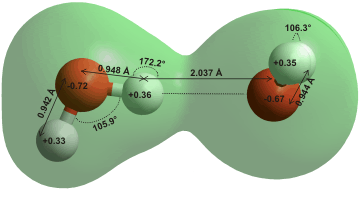
\includegraphics{images/h402}
}
\caption{The most energetically favourable water dimer calculated from first
  principles. \citep{watermolecule}}
\label{fig:dimer}
\end{figure}

\begin{figure}[h]
\centering
\resizebox{0.5\textwidth}{!}{
  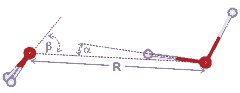
\includegraphics{images/dimr}
}
\caption{Water dimer angles. $R = 2.976\AA, \alpha = 6 \pm 20\degree, \beta =
  57 \pm 10\degree$. \citep{watermolecule}}
\label{fig:dimer-angle}
\end{figure}

The previously discussed predictors work well in the setting of general point
clouds, but in a point cloud consisting of water molecules we can create
predictors tailored towards water.

A water dimer is two water molecules loosely bonded by a hydrogen atom. This
is the simplest model for hydrogen bonding in water, and as such has been
extensively studied.

The oxygen which is loosely bonded to the hydrogen is expected to be
$2.976\AA$ away from the other oxygen. It is also expected that the vector
created by the O-H bond to be roughly in line with the vector of the loose O-H
bond \citep{watermolecule}. See Figure \ref{fig:dimer} and Figure
\ref{fig:dimer-angle}.

\subsection{Using the Model in Point Cloud Compressors}

\citep{omeltchenko2000sls} only exploit the fact that there may be many dense
clusters in MD simulations. It is more general than water compression, and
modifying it to use the relative layouts of the water molecules is not clear.

The predictors of \citep{merrycomp} and \citep{gumholdcomp} do not exploit the
layout of water molecules. Using water dimer model prediction can be done
given the positions of a water molecules atoms. The creation of the spanning
tree would be different, since we know the expected degree of the verticies is
at most two.

\begin{table}[t]
\centering
\resizebox{\textwidth}{!}{
\begin{tabular}{||l|c|c||}
  \hline
  \emph{Attribute/Method} & \citep{omeltchenko2000sls} & \citep{gumholdcomp} \\

  \hline

  \emph{Structure} & MD Simulation & Surface \\

  \emph{Progressive} & Single-rate & Single-rate \\

  \emph{Quantisation} & Yes & Yes \\

  \emph{Connectivity} & Space Filling Curve & Spanning Tree \\

  \emph{Exploits} & Dense/regular clusters & Regularity of scans \\

  \emph{Scope} & Global & Local \\

  \emph{Topology} & Geometry & Both \\

  \hline
  \hline

  \emph{Attribute/Method} & \citep{chen2005lcp} & \citep{devillers2000gci} \\

  \hline

  \emph{Structure} & 3D Model & Mesh \\

  \emph{Progressive} & Single-rate & Progressive \\

  \emph{Quantisation} & No & Yes \\

  \emph{Connectivity} & Spanning Tree & kd-trees \\

  \emph{Exploits} & Differential Coding & kd-tree properties \\

  \emph{Scope} & Global & Global \\

  \emph{Topology} & Connectivity & Neither \\

  \hline
  \hline

  \emph{Attribute/Method} & \citep{merrycomp} & \\

  \hline

  \emph{Structure} & Surface & \\

  \emph{Progressive} & Single-rate & \\

  \emph{Quantisation} & Yes & \\

  \emph{Connectivity} & Spanning Tree & \\

  \emph{Exploits} & Rectilinear scans & \\

  \emph{Scope} & Local & \\

  \emph{Topology} & Both & \\

  \hline
\end{tabular}
}
\caption{Taxonomy of the different methods.}\label{tab:taxonomy}
\end{table}


\section{Taxonomy of Techniques}

Refer to Figure \ref{tab:taxonomy} for an overview of the categorisations of
the different papers. There are two underlying philosophies which the
compression algorithms exploit, the \emph{scope} and the \emph{topology}.

\emph{Scope} is whether the algorithm is exploiting \emph{global} or
\emph{local} properties of the points. \citep{merrycomp} uses a local scope
since it exploits nearby points to predict the location of the current
point. \citep{chen2005lcp} uses a global scope, since it is trying to minimise
a global property of the spanning tree.

\emph{Topology} is whether the algorithm is trying to exploit connectivity or
geometric information. \citep{gumholdcomp} exploits both, but the geometry
more since it uses a predictor to predict the location based on other points
location. \citep{chen2005lcp} just tries to choose the best possible spanning
tree, so they exploit connectivity of points.

The other properties listed in the taxonomy are \emph{structure},
\emph{progressive}, \emph{quantisation}, \emph{connectivity} and
\emph{exploits}.

\begin{itemize}
\item \emph{Structure} is what type of point cloud the compressor targeting.

\item \emph{Progressive} is whether the compressor is a single-rate encoder or
  progressive encoder.

\item \emph{Quantisation} is whether the compressor applies quantisation
  before compression.

\item \emph{Connectivity} is how relationships between points are derived or
  modelled.

\item \emph{Exploits} is what the compressor is targeting for good
  compression.
\end{itemize}


\section{Summary}

The water dimer model gives a good predictor for exploiting the local
structure of water molecules. So using a predictive point cloud encoder
similiar to \citep{merrycomp} and \citep{gumholdcomp} should result in good
compression of water molecules.

Compressing the other atoms will require a more general technique. Using the
best point cloud compressor on the other atoms combined with the water
prediction scheme should result in better compression.


\chapter{Design and Implementation}

This chapter outlines the design and implementation of our compressor and
decompressor. The compression techniques investigated only cover intra-frame
compression. Intra-frame compression is where compression occurs per frame
independently of the other frames. Reference implementations of other schemes,
inter-frame compression as well as visualisation is also implemented, as such
the design needs to take into account these uses. Components outside of the
scope of intra-frame compression will not be covered in detailed.

The main contribution of this report is a predictive encoder targeting water
molecules. The compressor is referred to as the Water Compressor.

\section{Overview}

Compression is done on the DCD/PDB format, which is a format for storing MD
simulations. DCD files are explained in Section \ref{sec:molec-dynam-form}.

A high-level overview of how data flows in the compressors is illustrated by
the following: \todo replace with pretty picture similiar to the FBI
fingerprint compression paper

\[ DCDFile \to Atoms \to QuantisedAtoms \to Compressor \]

The decompressor works in the reverse direction:

\[ Decompressor \to QuantisedAtoms \to DCDFile \]

The decompressed DCD files are an approximation due to quantisation. Excluding
the quantisation step, the schemes are lossless. Note that each step in the
compression phase has auxillary information. The auxillary information is
required for reconstruction.

Reference implementations of \citep{devillers2000gci}, \citep{gumholdcomp} and
\citep{omeltchenko2000sls} are also implemented. These use the I/O and
quantisation components. Julian Kenwood implemented
\citep{omeltchenko2000sls}, while Keegan Carruthers-Smith implemented
\citep{devillers2000gci} and \citep{gumholdcomp}. Visualisation uses the I/O
and quantisation components as well and was implemented by Min-Young Wu.


\subsection{Dependencies}

All development was done on Linux, but no Linux or POSIX specific APIs where
used. The implementations should be cross platform, but have not been tested
on anything but Linux.

\paragraph{C++}
C++ fits the requirements of the project since the compressors need to be fast
and all the authors are competent in C++. Development was done with GCC 4.x.

\paragraph{ANN}
ANN is a library for approximate nearest neighbor searching. It is used to
speed up graph creation where locality of points is important. \citep{ann}

\paragraph{VMD DCD Loader Plugin}
This plugin is used to read and write DCD files. \citep{vmd}


\section{Components}
\label{sec:components}

A component-based approach was used to design the compressor and
decompressor. This is because the algorithm can be broken up into distinct
steps.

\todo picture showing components and who did what

The different components are the following:

\paragraph{Simulation I/O}

These components handle I/O to and from the simulation data files. The VMD DCD
loader plugin is used to load and write the DCD files. Implemented is also a
PDB reader for determining what each atom is in the DCD file. DCD is used
since it is the prevalent format used for storing simulation data, and it is
well supported in VMD.


\paragraph{Arithmetic Coder}

The water compression scheme as well as the point cloud schemes use arithmetic
encoding for encoding the residuals and tree. The usual approach of the
implementation of the arithmetic coder is used, where the encoder and the
model are separated.

The range of the residuals in the predictive schemes as well as the number of
different residuals is not known before hand. As such we use a novel approach
for an adaptive arithmetic model. We use an approach similiar to the technique
by \citep{cormack1984algorithms} used in Adaptive Huffman Encoding. The
adaptive model initially only has one symbol meaning ``new'' symbol. When
encoding if there is a new symbol, the ``new'' symbols is encoded followed by
a raw representation of the new symbol. By using a trie and a modification of
a Fenwick tree, insertion of new symbols into the model is $O(n \log n)$ where
$n$ is the number of seen symbols.

The encoder by \citep{omeltchenko2000sls} does not make use of an Arithmetic
Coder, instead it uses its own entropy coder. Every other encoder uses the
arithmetic encoder.


\paragraph{Quantiser}

The quantiser is responsible for quantising and dequantising a frame. The
quantiser takes in as input a number $b$. The quantiser quantises each
dimension independently using linear quantisation. The number of cells it
divides each dimension into is $2^b$. So after quantisation each coordinate
becomes a $b$-bit integer.

Linear quantisation is chosen since the water compressor (as well as the other
predictive compressor) require locality of the points to be
preserved. Quantisation is also necessary since small differences in
predictive residuals should be treated as the same for better entropy
encoding.

Converting the floating point values to integers introduces error. But for the
predictive schemes to be effective it is necessary. This is the only step
which is lossy. In the literature if the only lossy step is quantisation, the
algorithm is still referred to as lossless.


\paragraph{Permutations}

When decompressing we need to recover the atoms in the same order they are
listed in the original DCD file. The water compressor as well as the other
predictive point cloud schemes do not recover the original order. How
permutations are encoded is explained in Section \ref{sec:compr-perm}.


\paragraph{Compressors}

The compressor component is different for each compressor. It implements the
encoding and decoding of the quantised frames. The intra-frame compressors
which are implemented are the water compressor and reference implementations
of \citep{omeltchenko2000sls}, \citep{gumholdcomp} and
\citep{devillers2000gci}.


\paragraph{Verifiers}

Verifiers are for testing whether a compression scheme is working. Given a DCD
file and a decompressed DCD file, if the files match when quantised then the
compressor is working. There is the possibility of floating point error
causing a mismatch when the files are equivalent. This happens infrequently,
so the frames which do not match can be inspected manually to see if they are
the same.


\section{Compressing Permutations}
\label{sec:compr-perm}

Every compression algorithm explored in this report does not necessarily
preserve the order of the points when decompressed. For example in
\citep{devillers2000gci}
\[ (1, 2), (1, 3), (0, 0), (2, 3), (2, 2), (0, 2), (1, 1) \]
when decompressed becomes
\[ (0, 0), (1, 1), (0, 2), (1, 2), (1, 3), (2, 2), (2, 3) \]

When decompressing we need to recover the original order of the points, since
the index of a point indicates which atom it is in the DCD file format.

We experimented with five different types of permutation compressors. Each
permutation compressor takes in a permutation of $[0,1,\dots,N-1]$ and encodes
it to the file. Let the permutation be $[P_0, P_1, \dots P_{N-1}]$. The
decompressor then recovers the permutation.

\paragraph{Null}
Null does not write anything to the file. The decompressor just outputs the
order permutation $[0,1,\dots,N-1]$. A compressor which uses the null
compressor does not preserve the order. Every other permutation compressor
should do worse than this.

\paragraph{Na\"{\i}ve}
Na\"{\i}ve writes the permutation list straight to the file. Each index is
stored as a $32$-bit integer. Every other permutation compressor should do
better than this.

\paragraph{Delta}
Delta transforms the permutation into a list $L$, where $L_0 = P_0$ and $L_i =
P_i - P_{i-1}$ for $0 < i < N$. Arithmetic encoding is then done on $L$. $L$
is then written to file.

Decompression gets back the list $L$. Since $P_0 = L_0$ and $P_i = L_i +
P_{i-1}$ for $0 < i < N$ we can recover the original permutation. Since each
$P_i$ depends only on previous $i$'s, calculating $P_i$ in increasing order of
$i$ will recover $P$.

\paragraph{Interframe}
Interframe transforms the permutation $P$ into a list $L$. Let $P'$ be the
permutation from the previous frame. If it is the first frame, let $P' =
[0,1,\dots,N-1]$. Then $L_i = P_i - P'_i$ for $0 \le i < N$. Use arithmetic
encoding on $L$ and then write $L$ to file.

Decompression recovers the list $L$. Since $P_i = L_i + P'_i$, $P$ can be
recovered. Note that this method requires frames to be decompressed in order.

\paragraph{Optimal}
Optimal uses a static arithmetic coder with a frequency of $1$ for each
$P_i$. Since each $P_i$ occurs only once, this gives the best possible
compression.

A static arithmetic encoder model uses a Fenwick Tree to update the symbol
table after each encoding. This takes $O(\log(N))$ per update. In the optimal
permutation compressor we can get this down to $O(1)$ by using the fact that
we only ever encode each $P_i$ once. To encode a symbol $i$ the arithmetic
encoder requires $S_{tot}$, $S_i$ and $S_{i-1}$. $S_{tot}$ is the sum of all
the frequencies. $S_i$ is the sum of the frequencies for all the symbols less
than or equal to $i$. Since the frequency of each index is one, $S_i = i$ and
$S_{tot}$ is the number of permutations left. We need a way to map permutation
indicies to symbols which is quick to update once an index has been
encoded. The following algorithm is used:

\begin{verbatim}
init(permutation):
  number_of_symbols = permutation.size
  for i in 0, 1, ..., permutation.size - 1:
    index_to_symbol[i] = i
    symbol_to_index[i] = i
\end{verbatim}

\begin{verbatim}
pop_index(index):
  number_of_symbols--

  symbol = index_to_symbol[index]
  index2 = symbol_to_index[number_of_symbols]

  index_to_symbol[index2] = symbol;
  symbol_to_index[symbol] = index2;

  return symbol;
\end{verbatim}

\begin{verbatim}
pop_symbol(symbol):
  index = symbol_to_index[symbol]
  pop_index(index)
  return index
\end{verbatim}

To encode $P_i$, we encode $pop\_index(P_i)$. To decode, we return
$pop\_symbol(val)$ where $val$ is a value returned from the arithmetic
decoder.

The optimal permutation encoder is optimal in the general case. If we have $M$
indicies left to encode, each unseen index has probability $\frac{1}{M}$ of
occurring and every seen index has probability $0$ of occurring. So for each
$i$ we have that $S_{tot}=M, S_i = i, S_{i-1} = i-1$. This gives a probability
of $\frac{i-(i-1)}{M} = \frac{1}{M}$.

If there are $M$ indicies left, the lower-bound on the number bits to encode
an index is $\log_2(M)$. So if $P$ has $N$ indicies a lower-bound on the
number of bits to encode $P$ is
\begin{equation}
  \displaystyle\sum^{N}_{i=1} \log_2(i)
  \label{eq:optimal-lowerbound}
\end{equation}
Each index can fit into $\lceil\log_2(N)\rceil$ bits, so this is used as an
effective upper-bound. See Table \ref{tab:optimal-lowerbound} for values of
Equation (\ref{eq:optimal-lowerbound}) in bytes. Notice how as the size of the
permutation increases, the gains made by the optimal scheme decrease.


\begin{table}
  \center
  \resizebox{\textwidth}{!}{
  \begin{tabular}{|l||r|r|r|r|r|r|r|}
    \hline
    \emph{Permutation Size} & $1$ & $2$ & $10$ & $1000$ & $10\,000$ &
    $100\,000$ \\
    \hline
    \emph{Lower-Bound} & $0.00$ & $0.12$ & $2.72$ & $1066.17$ & $14807.26$ &
    $189588.02$ \\
    \emph{Effective Upper-Bound} & $0.00$ & $0.25$ & $5.00$ & $1250.00$ &
    $17500.00$ & $212500.00$ \\
    \emph{Percentage Gain} & $0.00$ & $33.33$ & $29.47$ & $7.94$ & $8.33$ &
    $5.70$ \\
    \hline
  \end{tabular}
  }
  \caption{Number of bytes needed for storing permutations of different
    sizes. See Equation (\ref{eq:optimal-lowerbound}) for the lower bound. The
    effective upper-bound is
    $\lceil\log_2(N)\rceil/8$} \label{tab:optimal-lowerbound}
\end{table}


\section{Water Compressor}

This section details the algorithm of the water compressor and is the main
contribution of this report. The encoder is implemented as a compressor
component and uses the components detailed in the Section
\ref{sec:components}.

The compressor processes each quantised frame in order. This encoder is a
predictive intra-frame encoder, and as such only compresses using information
contained in the frame.

The algorithm is similiar to the predictive point cloud compressors of
\citep{gumholdcomp} and \citep{merrycomp}. The following is a high level
overview of the algorithm:

\begin{verbatim}
CompressFrame(list_of_atoms_in_frame, arithmetic_encoder):
  list_of_water_molecules = FindWater(list_of_atoms_in_frame)
  list_of_other_atoms = FindNonWater(list_of_atoms_in_frame)
  compress(list_of_other_atoms, arithmetic_encoder)
  water_graph = CreateGraph(list_of_water_molecules)
  spanning_tree = CreateSpanningTree(water_graph)
  TreeSerialise(spanning_tree, arithmetic_encoder)
\end{verbatim}

\noindent Similarly decompression uses this algorithm:

\begin{verbatim}
DecompressFrame(arithmetic_decoder):
  list_of_other_atoms = decompress(arithmetic_decoder)
  list_of_water_atoms = TreeDeserialise(arithmetic_decoder)
  return list_of_other_atoms + list_of_water_atoms
\end{verbatim}

\todo once we get more substantial results we can pick which point cloud
compressor to use

An explanation of each step follows, along with motivation of why each step is
done.


\subsection{Finding Water Molecules}

The PDB file associated with a DCD file contains information on which atoms a
given atom is bonded to. Using the PDB file the encoder finds all oxygen atoms
which are bonded to two hydrogen atoms. This section was implemented in the
Simulation I/O component.

The implementation returns two lists: a list of water molecule indicies and a
list of other atom indicies. Every water molecule is specified as the indicies
in the frame of its corresponding oxygen and hydrogen atoms. Every index which
is not in a water molecule is stored in the second list.

The splitting between water molecules and other atoms is done so that
compression of water molecules and the other atoms can be done using different
encoders. The water compression predictors target water atoms, so a more
general compression method is used on the other atoms.


\subsection{Water Predictors}

The predictors are based on the models of water dimers explained in the
background chapter. There are three predictors used, the constant predictor
and the two hydrogen predictors.

Let $O, H_1, H_2$ be the predictions for where the water molecule will be and
let $O', H'_1, H'_2$ be the water molecules parent.

\paragraph{Constant Predictor}
The constant predictor predicts $O$ to be at $O'$. This predictor is included
since occasionally the hydrogen bond is broken (molecule information remains
static from the start of the simulation). If the bonds are broken the hydrogen
predictors are far less accurate than the constant predictor.

\paragraph{Hydrogen Predictor}
The hydrogen predictor predicts along $O'-H'_1$ or $O'-H'_2$. We simplify the
model in Figure \ref{fig:dimer-angle} and assume $\alpha$ is $0\degree$. Then
$O$ is predicted to be at $O' + 2.976\frac{O'-H'_i}{|O'-H'_i|}$.

In all three prediction schemes $H_1$ and $H_2$ are predicted to be at
$O$. This is since their is a large variability in $\beta$ in Figure
\ref{fig:dimer-angle}.


\subsection{Creating the Water Graph}

Creating the spanning tree is $O(E \log E)$, where $E$ is the number of edges
in the graph. When creating the spanning tree, each molecule's predictions are
compared to all of its neighbours. If the graph created is the complete graph,
$E$ is $O(N^2)$, where $N$ is the number of water molecules. This is too
inefficient for large scale simulations.

So the purpose of graph creation is to efficiently minimise the degree of the
verticies (and hence $E$), while maintaining the neighbours which predict well
against the predictors.

The neighbours which predict well against a water molecule are related to the
spatial locality of the oxygens. So the approximation used is to add edges
between all molecule pairs where the oxygens are within $3\AA$. The degree of
a vertex is then a small number (typically less than 5 from
experimentation). The number of edges created is usually $O(N)$.

The na\"{i}ve implementation of graph creation would compare each molecule
against every other yielding a $O(N^2)$ algorithm. This is too slow. Instead a
kd-tree is used to create the graph. The kd-tree is populated with the oxygen
positions. Then using ANN's approximate fixed radius search one can find all
other oxygens within approximately $3\AA$. Creating the graph requires $O(N
\log N)$ time. The fixed radius search takes approximately $O(\log N)$
time. The search is done per molecule, so the overall time complexity for
graph creation is $O(N \log N)$. The algorithm is as follows:

\begin{verbatim}
createGraph(list_of_water_molecules):
  graph = graph of water molecules
  kdtree = KDTree(list_of_water_molecules.O_pos)
  for cur_mol in list_of_water_molecules:
    radius = 3 angstroms
    for mol in kdtree.fixed_radius_search(cur_mol.O_pos, radius):
      graph.addEdge(cur_mol, mol)
  return graph
\end{verbatim}



\subsection{Creating the Spanning Tree}

The order in which the points are serialised, and which predictor is used for
each point is not obvious from the graph created in the previous section. A
directed tree is created from the graph since each molecule is predicted by
one other molecule. The edge $O' \to O$ indicates that $O$ is predicted using
the position of $O'$.

The graph is not necessarily connected, so a spanning tree is created for each
component. A root vertex is arbitrarily selected. Then each tree in the forest
is connected to the root with the constant predictor. Each edge $O' \to O$ is
labelled with what predictor is used to predict $O$ from $O'$.

For each component a root is arbitrarily picked. The tree is then created by
using a modification of Dijkstra. The priority queue stores potential edges,
and sorts by the residual from the prediction. When a potential edge $O' \to
O$ is removed from the queue, it is added to the spanning tree if $O$ is not
already in it. The algorithm is illustrated by the following:

\begin{verbatim}
create_spanning_component(graph, tree, component_root, root):
  priority_queue q
  q.add(0, component_root -> root, constant)
  while q not empty:
    residual, v' -> v, p = q.pop()

    if v not in tree:
      tree add edge v' -> v with predictor p

    predictions = { constant_predictor(p),
                    h1_predictor(p),
                    h2_predictor(p) }

    for u in graph[v].children:
      if u in tree:
        continue

      residual, predictor = smallest_residual(u, predictions)

      q.add(residual, v -> u, predictor)
\end{verbatim}

This algorithm is $O(E \log E)$ since for every edge in the graph, a potential
edge is added to the queue. In the implementation an optimisations is used
which reduces the complexity to approximately $O(N \log E)$. The smallest seen
residuals is kept for each molecule. Then a potential edge $v \to u$ is only
added if the residual is less than the current smallest residual for $u$.


\subsection{Tree Serialisation}

This stage encodes the predictions and spanning tree. The predictions are
encoded in breadth first order. The spanning tree is also encoded since it is
required to reconstruct what each molecule is predicted from. The BFS then
starts at the root of the spanning tree and for each molecule in the BFS the
following happens:

\begin{verbatim}
process(O' -> O, predictor):
  prediction  = prediction(O', predictor)
  O_residual  = water_molecule.oxygen - prediction
  H1_residual = water_molecule.hydrogen1 - water_molecule.oxygen
  H2_residual = water_molecule.hydrogen2 - water_molecule.oxygen

  residual_encoder.encode({ O_residual, H1_residual, H2_residual })
  permutation_encoder.encode(water_molecule.index)

  for pred, child in O.children:
    tree_encoder.encode(pred)
    bfs_queue.push(O -> child, pred)
  tree_encoder.encode(sentinel)
\end{verbatim}

The root does not have a predictor, so by default the constant predictor will
predict the position to be $(0,0,0)$.


\paragraph{Deserialisation}

The tree deserialisation is the reverse of the serialisation. It populates a
quantised frame with the following algorithm:

\begin{verbatim}
q = queue()
q.push(NULL, constant_predictor)

while q not empty:
  parent, predictor = q.pop()

  prediction  = predict(parent, predictor)
  O_position  = residual_decoder.decode() + prediction
  H1_residual = residual_decoder.decode() + O_position
  H2_residual = residual_decoder.decode() + O_position

  index = permutation_decoder.decode()
  water_molecules[index].oxygen    = O_position
  water_molecules[index].hydrogen1 = H1_position
  water_molecules[index].hydrogen2 = H2_position
\end{verbatim}



\chapter{Random sections to be integrated properly}

\section{Future Work}

\paragraph{Parallelism}

The intra-frame compressor works independently of each frame. This allows
parallising over frames.

\paragraph{General Molecular Dynamics Predictors}

Running an approximate simulation and using the positions it obtains as
predictors should give good general predictors. This also does not need to
store the permutation information.

\paragraph{Better joining of components in spanning tree}

The water compressor implementation joins up the components by adding an edge
to a route. Explore ways of joining up better. Possible ways include using a
MST of the components or encoding the components separate to the errors.

\nocite{*}
\bibliography{report_keegan}

\end{document}

% LocalWords:  oxygens Deserialisation deserialisation BFS
